\section{Design and Architecture}


\subsection{Model-View-Controller Architecture}

The Model–view–controller (MVC) is a software design pattern[TODO] which goal is to enhance the modularity, maintainability, and scalability of our system. It separates the application into three layers, distinct components:

\begin{enumerate}
	\item the \textbf{model} which is the representation of the informations and represented by the Database;
	\item the \textbf{view} which is the presentation layer that display the informations and interact with the user;
	\item the \textbf{controller} which is the link between the 2 previous one but also the processing layer.
\end{enumerate}


\subsection{Data model}

A new architecture has been conceived to accommodate the expanded scope of the project. Unlike the previous iteration, which focused primarily on basic employee information management such as names, email addresses, and phone numbers, the revised architecture will encompass a broader range of functionalities. This expanded scope includes the capability to create and manage contracts, as well as managing all the projects within the organization.


%\newpage

%\begin{landscape}
%	\begin{figure}[h!]
%		\centering
%		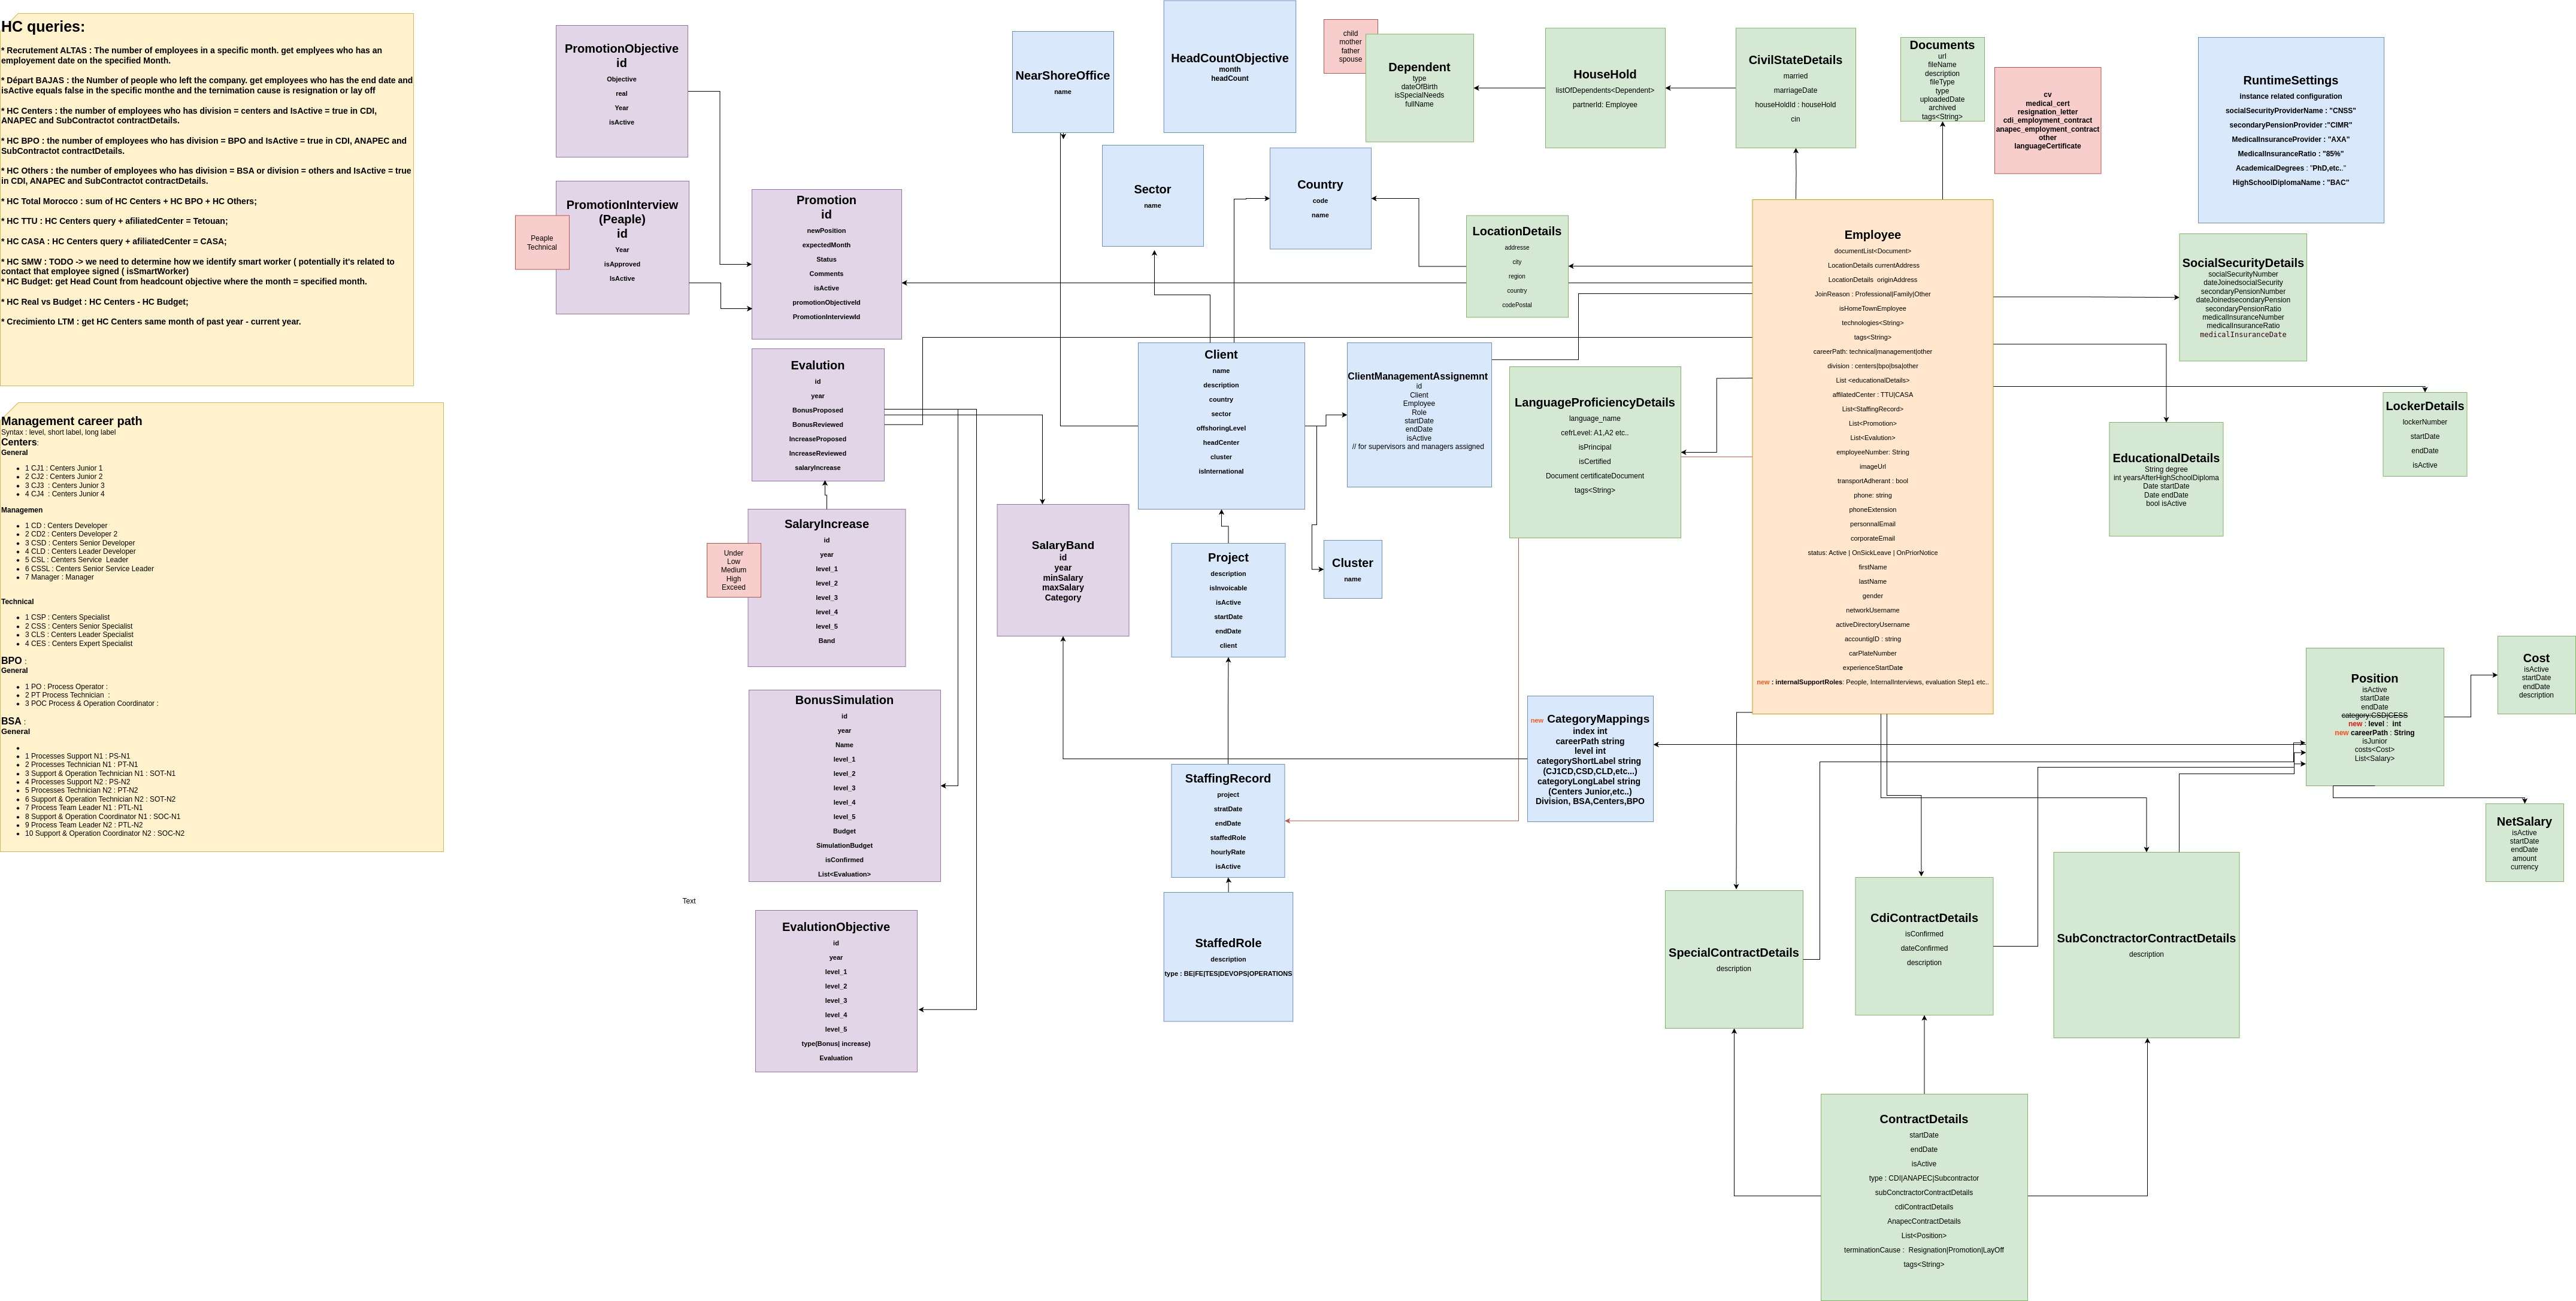
\includegraphics[width=1.65\textwidth]{Image/architecture.jpg}
%		\caption{Diagramme d'architecture du système}
%		\label{fig:architecture_diagram}
%	\end{figure}
%\end{landscape}

\begin{figure}[h!]
	\centering
	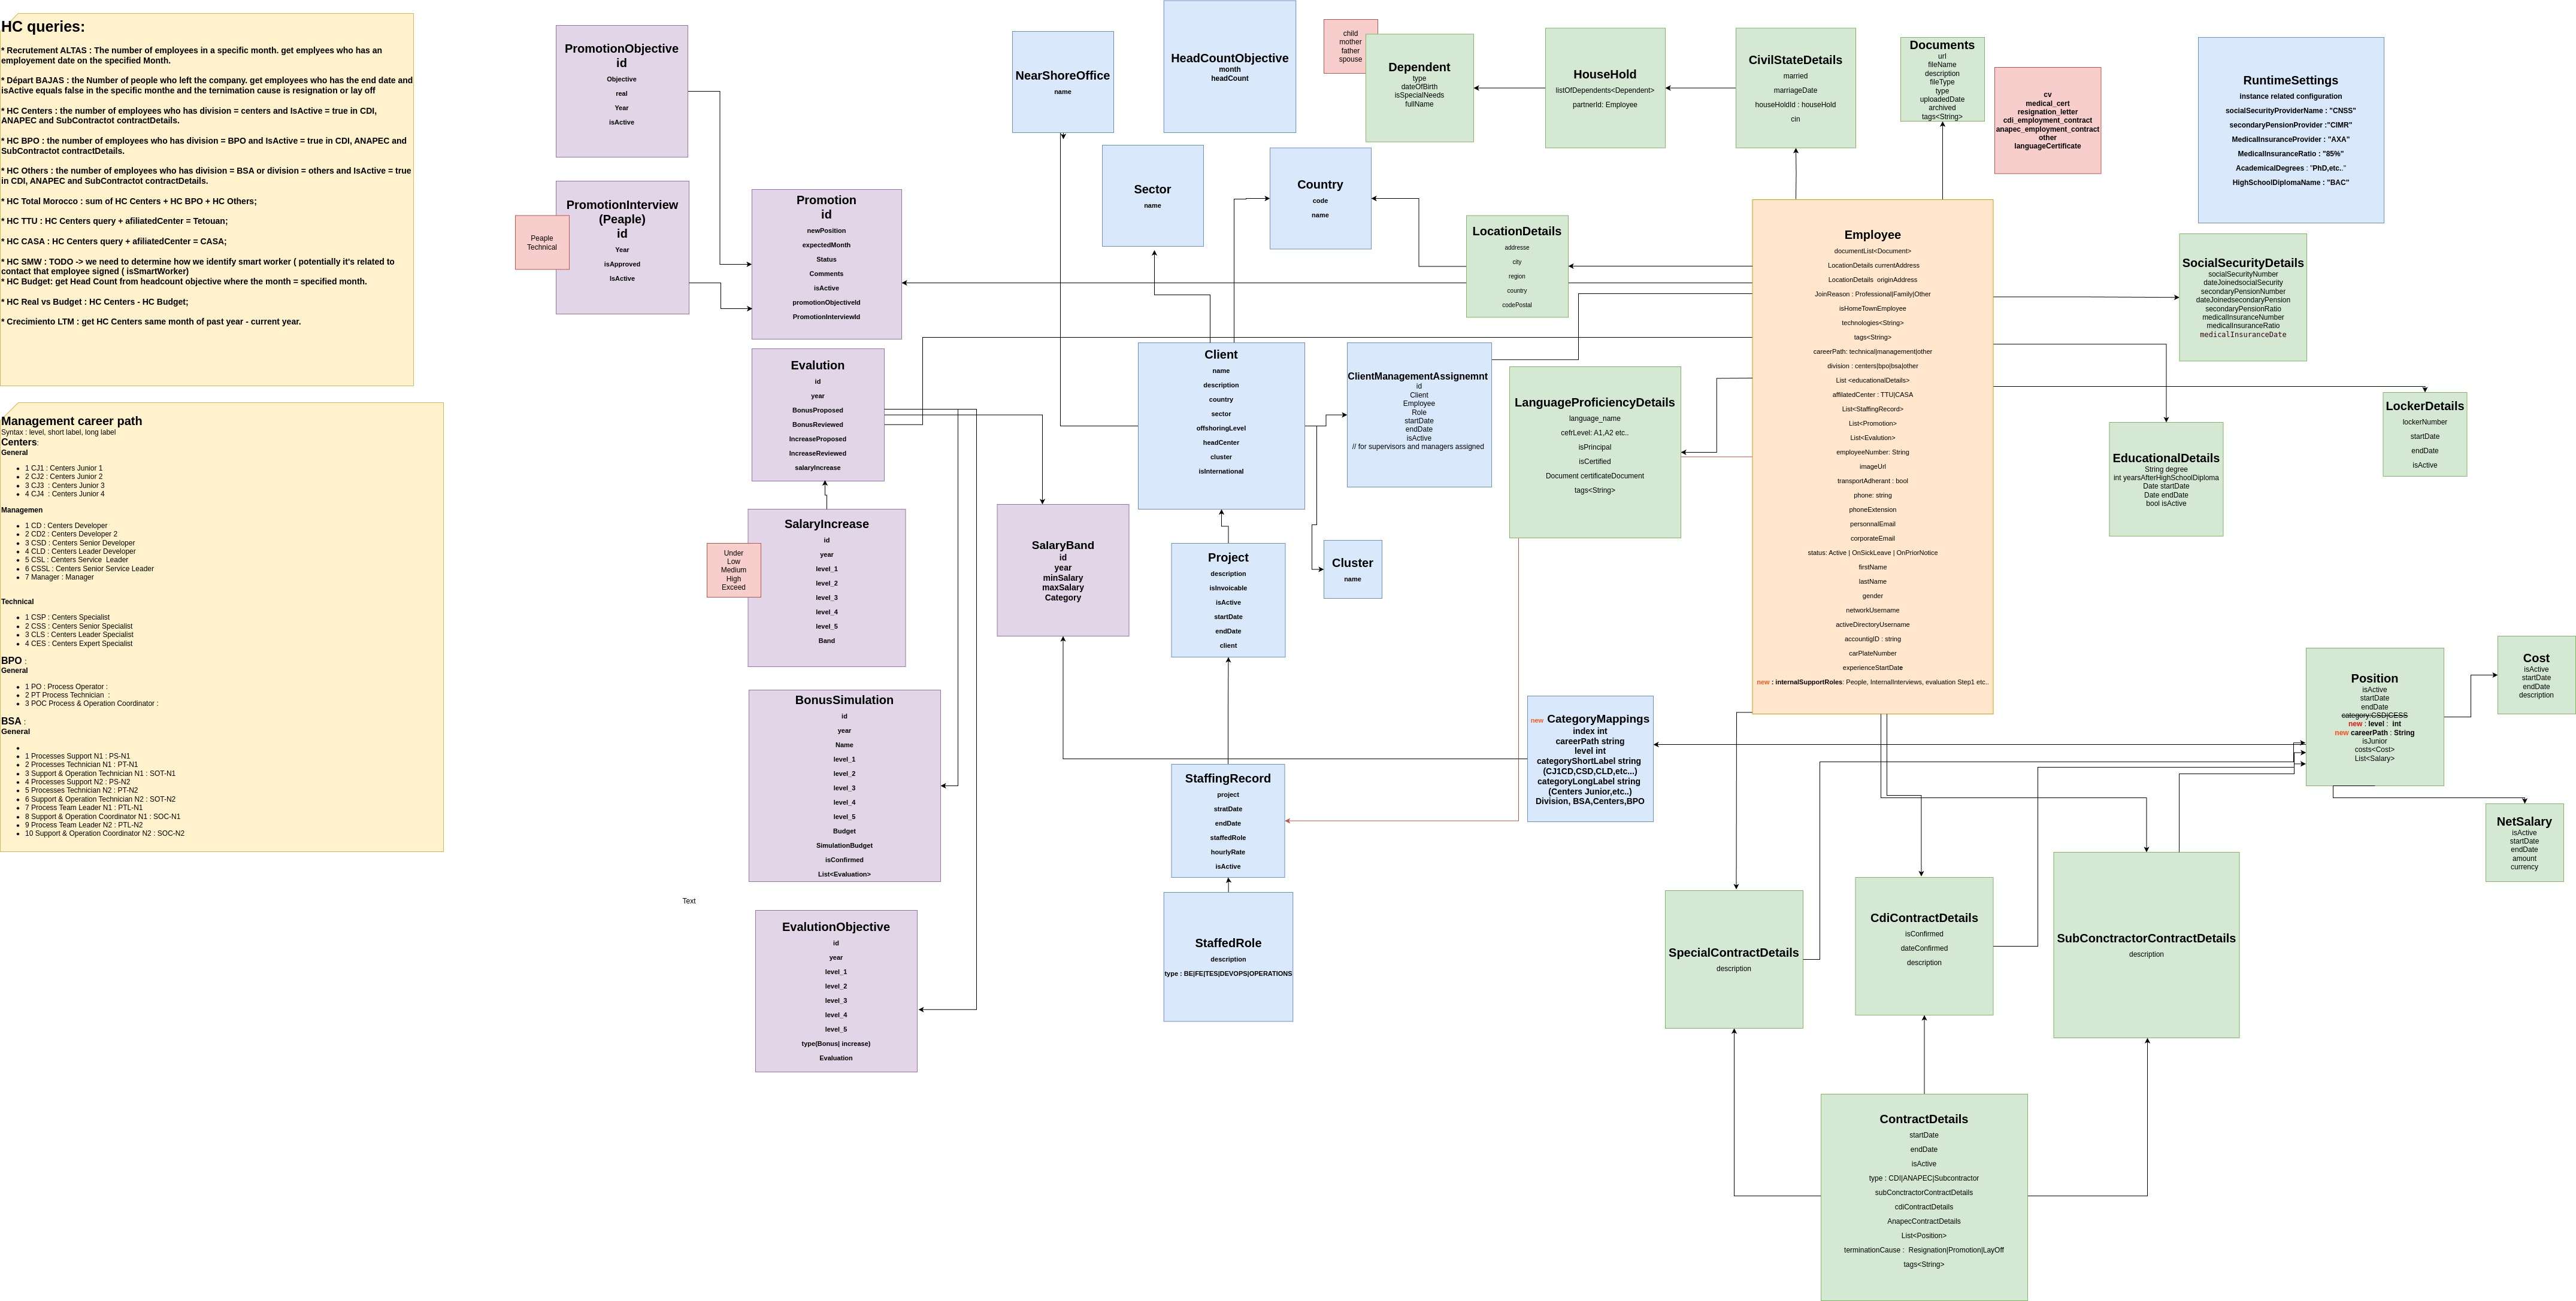
\includegraphics[width=0.8\textwidth]{Image/architecture.jpg}
	\caption{Diagramme d'architecture du système}
	\label{fig:architecture_diagram}
\end{figure}

\newpage

\subsection{Servers}

We have multiples servers, that we can manage throught Heroku[TODO], located in Amazon Web Service (AWS) cloud:

\begin{itemize}
	\item one for the Angular front-end (view layer);
	\item one for the Java back-end (controller layer);
	\item one for the PostgreSQL database (model layer).
\end{itemize}

\subsection{Authentication}

Our application requires authentication to be accessed. For thus we use Azure Active Directory (Azure AD) to provide secure and efficient identity management. It is a comprehensive cloud-based identity and access management solution that helps our organization manage user identities and control access to resources.
Additionally, Azure AD can be integrated seamlessly in the applications and services which make it a good way to secure the access of our application.


\subsection{Technologies}

\subsubsection{Back-end}

The language Java has been chosen for our application. Firstly because the previous application was already made with but also because it is known for its portability across different operating systems, Java enables our applications to run seamlessly in diverse environments without making any adjustment, which is particularly usefull as developpers use as well Windows, Mac and Linux. Its strong typing and object-oriented features help ensure code reliability and maintainability.\\

Additionally, Java includes a lot of libraries and frameworks that accelerates development and allows us to integrate a variety of efficient functionalities. More specifically, we are using Spring Boot [TODO]. This last one is an open-source framework that simplifies the development of our applications by providing a comprehensive set of features and tools. Spring Boot enables developers to implement commons functions [TODO mapstruct] and manage dependancy injection [TODO].




\subsubsection{Front-end}

For the front-end, Angular has been selected.



